Cholera is an acute intestinal infection causing severe diarrhea that may lead to dehydration, and sometimes death. The global burden of cholera is still high, around 3 million cases per year in endemic areas (e.g. in Haiti, Asia and Sub-Saharan Africa)~\cite{ali_updated_2015}. 
Recently, a political will to eliminate cholera has arisen. The World Health Organization (WHO) initiated a Global Task Force for Cholera Control (GTFCC), who aims at eliminating cholera by 2030\footnote{In this case, elimination is defined as a 90\% reduction of cholera deaths/year.}. There is a general consensus that, to reach this goal in endemic countries, there must be substantial improvements in education, sanitation, hygiene, medical treatment and prevention. Moreover, in the event of a cholera outbreak, timely interventions are crucial to limit the spread of the disease. With limited resources, public health officials face a number of challenging decisions, and a data driven decision support to guide the rational deployment of cholera control strategies is needed. Furthermore, on the road toward elimination, the need to setup context-specific tailored approaches appears. 

\section{A primer on cholera} 

Cholera is a waterborne infectious disease that causes an acute diarrhea in symptomatic individuals. However, most infected individuals are asymptomatic, i.e., they do not present symptoms. Since their mobility is not hindered, they become a vector of the infection. If not properly treated, cholera can kill children and adults within hours. The current cholera pandemic started in 1961, reached Africa in 1971 and the Americas in 1991~\cite{mutreja_evidence_2011}. The global burden of cholera is difficult to estimate. It remains high, with an estimated 2.86 million annual cases in endemics countries. The mortality is estimated at 95,000 deaths per year~\cite{ali_updated_2015}. In the following we highlight some relevant aspects about cholera transmission, while the biological and medical features of cholera are outside the scope of this report. 

\paragraph{Classification} Of the numerous strains of \emph{Vibrio cholerae}, only O139 and O1 cause disease epidemics. O1 caused all recent epidemic, and is divided in two serogroup: classical O1 and El Tor, which are both divided into two serotype: Ogawa and Inaba. Cholera classification has its importance as it affects all epidemiological characteristic (for example, El Tor survives longer in water and has an higher asymtomatic/symptomatic ratio)~\cite{who_cholera_2017}. The current cholera pandemic is mainly caused by El Tor, while some sporadic cases in Asia are caused by an O139 derivative. 

\paragraph{Transmission} An individual becomes infected through the ingestion of a critical dose of \emph{V. cholerae}~\cite{kaper_cholera._1995}. Two main exposure pathways fuel cholera transmission. First, discovered by John Snow during the 1854 London cholera outbreak, an \textit{indirect} exposure occurs from consumption of unsafe water contaminated by raw sewage~\cite{snow_mode_1855}. % Hom much ingestion 
\textit{Direct}, or human-to-human exposure occurs when bacteria are transmitted from an infected directly to a healthy person, for example via contaminated food.% In this case, environmental factors do not play a major role, except for possibly enhanced transmission due to crowding~\cite{boelee_options_2013}.


\paragraph{Symptoms} Once an individual has contracted the infection, symptoms may appear within 12 hours to 5 days~\cite{azman_incubation_2013}. Then, a wide range of outcomes are possible. Most of the time, the infection is inapparent, resulting in asymptomatic individuals. On the other end of the spectrum, severe infection occurs in 1\% to 15\% of the cases and leads to vomiting and profuse rice water diarrhea. Between asymptomatics and severe infections, there are many stages of mild infections that are difficult to quantify as symptoms are indistinguishable unless tested in a laboratory from those of numerous other infections causing diarrhea~\cite{king_inapparent_2008, kaper_cholera._1995, nelson_cholera_2009, van_de_linde_observations_1965, mccormack_community_1969}.  The severity of illness correlates with the number of \textit{V. cholerae} ingested~\cite{brouwer_dose-response_2017}, and depends on the cholera strain and personal characteristics immunity, pregnancy, blood type, ...~\cite{who_cholera_2017}. For severely infected individual, treatment is crucial: natural mortality can be up to 60\%, but a proper re-hydration therapy lowers mortality below 1\%~\cite{luquero_mortality_2016} .   


\paragraph{Shedding} The intensity of the shedding varies with the intensity of the infection. It goes from $10^3$ to $10^{9}$ vibrios per gram of stool for asymptomatic infected and severely infected individual respectively~\cite{nelson_cholera_2009}. Similarly, the duration of the diarrhea period typically ranges from a day up to two weeks~\cite{nelson_cholera_2009, kaper_cholera._1995}.
This suggests that asymptomatic individuals may be of great importance for cholera transmission. 

\paragraph{Immunity} Infected individuals that recover from the infection are immunized against the same \textit{V. cholerae} strain. The duration of acquired immunity is difficult to estimate, and depends on many factors. Acquired immunity has been reported to range from few months to several years, possibly depending on the virulence of the infection~\cite{levine_duration_1981, king_inapparent_2008, kaper_cholera._1995, woodward_cholera_1971, glass_seroepidemiological_1985, clemens_biotype_1991}.

\paragraph{Environmental reservoir} Once shed, \textit{V. cholerae} can survive in the environment for a long time, in particular in brackish waters and estuaries. There exist no marine host, but complex ecological association processes take place in the aquatic medium~\cite{reidl_vibrio_2002, bertuzzo_space-time_2008}. There is an ongoing debate about how long  \textit{V. cholerae} can survive in water and how much it can reproduce.

\paragraph{Reporting} WHO guidelines recommend that, when a patient enters a treatment center, his name, address, sex, age (over or below 5) and symptoms are recorded~\cite{who_first_2010}. The clinical definition of a suspected/confirmed cholera case varies. Usually, after more than three rice water stools in a day, a individual is diagnosed as suspected cholera case. Such diagnosis can be validated using rapid diagnosis tests (RTDs) and a more precise information is obtained through culture. Test results are not always available, especially during an outbreak. For this reason, after the first confirmed cholera case, each patient having diarrhea is reported as a suspected cholera case.  As a consequence, over-reporting during an outbreak situation is more likely than under reporting, which occurs, for example, when an individual cannot reach a treatment center.  % TODO: REF cite paper GTFCC

\paragraph{Climatic Drivers} There exists a complex but clear link between precipitation and cholera cases, as shown in Figure~\ref{rain}. For example, after hurricane Matthew and heavy rainfall in October 2016 a cholera epidemic started from few cases in Haiti~\cite{rinaldo_reassessment_2012, gaudart_spatio-temporal_2013}. Similarly, cholera in many African countries follows a seasonal trend, with the epidemiological curve raising during the rainy season~\cite{baracchini_seasonality_2017, pascual_cholera_2000}.  Rainfalls play a major role in water contamination, for instance through the washout of open-air defecation and raw sewage circulation in the environment.  % TODO citation crwoing in actrop

\begin{figure}
\centering
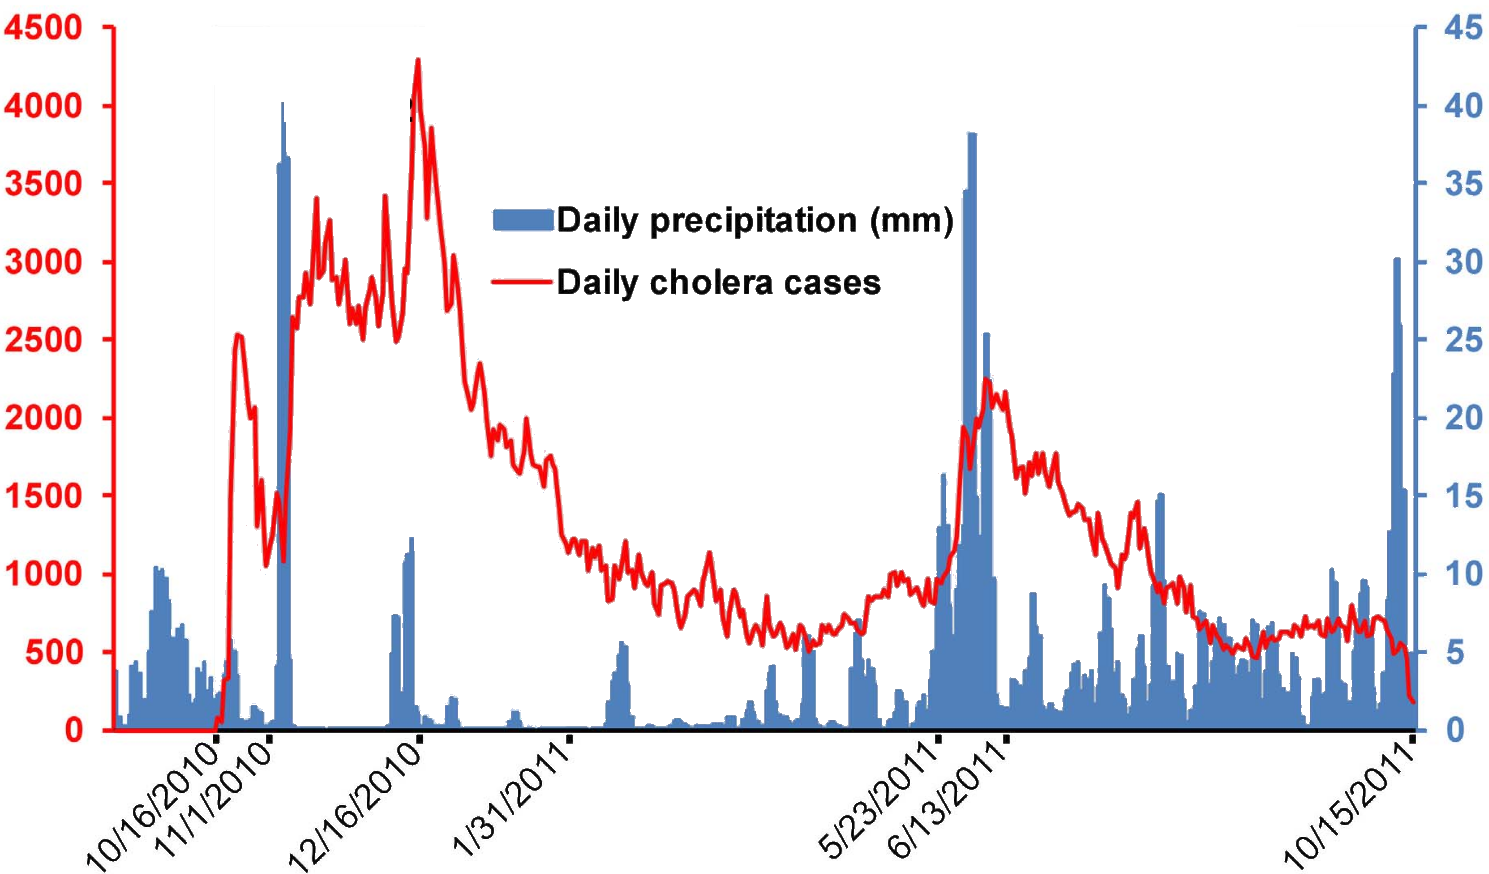
\includegraphics[width=.7\textwidth]{fig/cholera-rainfall.png}
\caption{Daily cholera cases (red), daily rainfall (blue), and epidemic phases (grey) in Haiti from September 15, 2010 to October
16, 2011. We observe a correlation between heavy rainfall event and case resurgence. From Gaudart \textit{et al.} \textbf{gaudart:spatio-temporal:2013}.}
\label{rain}
\end{figure}

Other climatic factors influence \textit{V. cholerae} survival and reproduction in water, and cholera transmission trough crowding effect~\cite{koelle_refractory_2005}.

\paragraph{Human mobility and hydrological transport} Spatial spread of cholera outbreaks occurs through two networks. \textit{V. Cholerae} in water may be transported through the river network. A famous example is the spread of the 2010 Haiti epidemic along the Artibonite river~\cite{gaudart_spatio-temporal_2013}. But more importantly, human mobility plays a major role in the spreading of the infections. The large number of shedding asymptomatic may transport and disperse cholera across a country or even worldwide.  Cholera was brought into Haiti by infected Nepalese soldiers. However, mobility, especially in humanitarian crisis situations often associated with cholera, remains difficult to predict~\cite{lu_predictability_2012, riley_large-scale_2007, bengtsson_improved_2011, rebaudet_dry_2013}.

\section{Cholera Modeling}
Cholera modeling has received a lot of attention since the 2010 Haiti outbreak, and serves different purposes. The ultimate goal being  the forecasting and estimating the propagation of uncertainties from the observable past to the future. Alongside, modeling helps us to understand the different processes of the cholera life cycle. As a substitute for physical experiments, different mechanistic pathways can be compared by benchmarking them against the reproduction of reported cases. %

Models may have only one spatial dimension or may consider the spatial spread of the epidemic across several nodes. Spatially-explicit mathematical models provide key insights into the course of an ongoing epidemic, where transmission is heterogeneous in space and time.

%%%%%%%%%%%%%%%%%%%%%%%%%%%%%%%%%%%%%%%%%%%%%%%%%%%%%%%%%%%%%%%%%%%%%%%%%%%%%%%%%%%%%%%%%%%% ok
\subsection{Spatially-explicit cholera model}
A spatially-explicit model has been developed at ECHO in the past 10 years~\cite{bertuzzo_space-time_2008}. Studies on the dynamics of several cholera epidemics, occurred in South Africa (2000)~\cite{mari_modelling_2012}, Senegal (2005), Haiti (2010-2016)~\cite{bertuzzo_prediction_2011}, Democratic Republic of the Congo  (2004-2011), stand as a significant proof of concept.  %TODO Missing ref

We present here a complete formulation of the model, including patterns and effectiveness of vaccinations, human and hydrological mobility~\cite{bertuzzo_probability_2016,pasetto_real-time_2017}

The model is a variation of the SIR model introduced first by Kermack and McKendrick~\cite{kermack_contribution_1927}, with additional compartments for the vaccinated individuals and the bacteria concentration in the environment.

The model subdivides the area potentially concerned by the epidemic into $n$ sub-regions. The sub-regions, defined by political boundaries or geomorphological features (like watersheds~\cite{bertuzzo_probability_2016}), are represented as connected nodes. The $n$ nodes represent $n$ human communities having population size $H_i$, $i=1,\dots, n$. 

At time $t$ and for each node $i$, the individuals in the node can be grouped into six compartments:

\begin{itemize}
\item $S_i(t)$: susceptible individuals  have no immunity, and may enter in contact with the bacteria and become infected (symptomatic or not),
\item $I_i(t)$: infected individual shed bacteria into the community reservoir,
\item $R_i(t)$: recovered are temporally immune, and don't participate in disease transmission,
\item $V^S_i(t)$: vaccinated susceptible,
\item $V^I_i(t)$: vaccinated infected,
\item $V^R_i(t)$: vaccinated recovered.
\end{itemize}

In addition, the model considers the bacterial concentration of \textit{V.~cholerae} in the water reservoir of the community, $B_i(t)$. The $n$ nodes are connected by both human mobility and pathogen transport through water.

Individuals commute from node $i$ to node $j$ with probability $Q_{ij}$. Bacteria are transported along the river network from node $i$ to node $j$ with probability $P_{ij}$, as shown in Figure~\ref{fig:bertuzzo14_SIRB}.


The cholera dynamics are described by the following set of coupled ordinary differential equations:
\begin{eqnarray}
\frac{dI_i}{dt} &=& \sigma F_i(t) S_i - (\gamma + \mu + \alpha) I_i \label{eq:I2}\\
\frac{dR_i}{dt} &=& (1-\sigma) F_i(t) S_i + \gamma I_i - (\rho + \mu+\frac{\nu_i(t)}{S_i+R_i}) R_i \label{eq:R2}\\
\frac{dV^S_i}{dt} &=& \nu_i(t) \frac{S_i}{S_i+R_i}-\mu V^S_i \label{eq:VS2}\\
\frac{dV^I_i}{dt} &=& \sigma (1-\eta) F_i(t) V^S_i - (\gamma + \mu + \alpha) V^I_i \label{eq:VI2}\\
\frac{dV^R_i}{dt} &=& \nu_i(t) \frac{R_i}{S_i+R_i} + (1-\sigma) (1-\eta) F_i(t) V^S_i + \gamma V^I_i - (\mu+\rho_v) V^R_i \label{eq:VR2}\\
\frac{dB_i}{dt} &=& - \mu_B B_i +\frac{p}{W_i}\left[1 + \phi J_i(t) \right] \left((1-m)(I_i +V_i^I)+m \sum_{j=1}^n Q_{ij} (I_j +V_j^I)\right)- \nonumber \\
&& l \left( B_i - \sum_{j=1}^n P_{ji} \frac{W_j}{W_i} B_j \right)
\end{eqnarray}
%
where the population~$H_i$ of each node is assumed to be at demographic equilibrium, thus $S_i=H_i-I_i-R_i-V_i^S-V_i^I-V_i^R$.

The force of infection, i.e the rate at which individual enters in contact with the diseases, is written as:
%
\begin{equation}
F_i(t) = \beta \left[ (1 - m) \frac{B_i}{K + B_i} + m \sum_{j=1}^n Q_{ij} \frac{B_j}{K + B_j} \right].
\label{force}
\end{equation}

The parameter~$\beta$ represents the maximum exposure rate, which may decrease in time due to awareness of the population on the cholera transmission factors~\cite{bertuzzo_probability_2016}. The fraction $B_{i}/(K+B_{i})$ is the probability of becoming infected due to the exposure to a concentration~$B_i$ of \textit{V.~cholerae}, $K$ being the half-saturation constant~\cite{codeco_endemic_2001}. The force of infection in a given node depends for a fraction ($1-m$) to the local concentration of \textit{V.~cholerae}, $B_i$, while the remaining fraction $m$, represents the community-level probability that individuals travel outside their node, accounts for the contribution of the concentration~$B_j$ of the remote communities. 
The human mobility is accounted with the matrix $Q_{ij}$ representing the probabilities that an individual living in node $i$ reaches~$j$ as a destination. Because of human mobility, a susceptible individual residing at node $i$ can be exposed to pathogens in the destination community $j$. 
In the lack of detailed mobility data,  the probabilities~$Q_{ij}$ can be estimated through a gravity approach~\cite{erlander_gravity_1990} to model human mobility:
%
\begin{equation}
Q_{ij} = \frac{H_j e^{-d_{ij}/D}}{\sum_{k \neq i}^n H_k e^{-d_{ik}/D}} \, ,
\label{eq:mob}
\end{equation}
%
where the attractiveness of node~$j$ depends on its population size $H_j$, while the deterrence factor is assumed to be dependent on the distance~$d_{ij}$ between the two communities via an exponential kernel (with shape factor~$D$).  

Due to the contact with contaminated water, a fraction $\sigma$ of the infected individuals develops symptoms, passing from compartment $S$ to $I$. The remaining fraction~$(1-\sigma)$ does not develop symptoms, does not contribute to the disease transmission, and is considered temporally immune, thus passing from compartment $S$ to $R$.  Symptomatic infected individuals recover at a rate~$\gamma$, or die due to cholera or other causes at rates~$\alpha$ or $\mu$, respectively.
Recovered individuals lose their immunity at rate~$\rho$, thus passing from compartments $R$ to $S$, or die at a rate~$\mu$.  % TODO Too many times property.

The environmental concentration of \textit{V.~cholerae} at a node $i$ may increase due to both human mobility and to hydrologic dispersion. Human contributions depends from a fraction $1-m$ on the local infected individuals and form a fraction $m$ on the symptomatic infected individuals moving according to the mobility model. The increase in bacteria concentration is modeled with the rate~$p/W_i$, where $p$ is the rate at which bacteria excreted by an infected individual reach and contaminate the local water reservoir of volume $W_i$ (assumed to be proportional to population size, i.e., $W_i=c H_i$ as in~\cite{rinaldo_reassessment_2012}) and $\mu_B$ is the rate of decay of \textit{V.~cholerae}. Bacteria undergo hydrologic dispersal at a rate~$l$: pathogens travel from node~$i$ to~$j$ with probability $P_{ij}$, which is assumed to be one if node~$j$ is the downstream nearest neighborhood $i$, and zero otherwise. In order to express the worsening of sanitation conditions caused by rainfall-induced runoff, when relevant, which causes additional pathogen loads to enter the water reservoir due to effects such as the overflow of pit latrines and washout of open-air defecation sites~\cite{gaudart_spatio-temporal_2013}, the contamination rate $p$ is increased by the rainfall intensity $J_i(t)$ via a coefficient $\phi$~\cite{rinaldo_reassessment_2012,righetto_rainfall_2013}. By introducing the dimensionless bacterial concentrations $B_i^*=B_i/K$,  it is possible to group three model parameters into a single ratio $\theta=p/(cK)$~\cite{bertuzzo_space-time_2008}.



The estimation of the local incidence is computed integrating over the new symptomatic individuals,
%
\begin{equation}
\frac{d C_i}{dt} \ = \ \sigma F_i S_i  \, , \label{eq:C}
\end{equation}

During the vaccination campaign, OCV doses are assumed to be distributed with rate $\nu_i(t)$ to susceptible and recovered individuals, which enter the compartments $V^S$ and $V^R$. As the OCV provides a partial immunity having efficacy $\eta$, $0\leq \eta \leq 1$, vaccinated susceptibles ($V^S$) can become infected ($V^I$) through a decreased force of infection of a factor $(1-\eta)$ with respect to non-vaccinated individuals. Vaccinated infected individuals behave exactly like infected ones, but are placed in a different compartment to exclude them from future vaccination campaigns. After recovering at  rate $\gamma$, they lose their vaccine protection at rate $\rho_{v}$.


%%%%%%%%%%%%%%%%%%%%%%%%%%%%%%%%%%%%%%%%%%%%%%%%%%%%%%%%%%%%%%%%%%%%%%%%%%%%%%%%%%%%%%%%%%%% ...
\subsection{Other cholera models}

Recently, cholera modeling has received a lot of attention. Mechanistic cholera models embed uncertainties into their parameter distribution, and differ in the way they account for the epidemiological processes~\cite{kirpich_controlling_2017, tuite_cholera_2011, chao_vaccination_2011, kirpich_cholera_2015}. For example, Einsenberg \textit{et al.} accounts for rainfall with a multiplicative effect on the force of infection~\cite{eisenberg_examining_2013, eisenberg_identifiability_2013, eisenberg_cholera_2013}. Most models are spatially implicit, however there have been a number of attempts to describe the spatial spread of the epidemic. For example, Andrew and Basu used an approach with isolated nodes and independent transmission parameters in each node~\cite{andrews_transmission_2011}.  Mechanistic models can be compared using formal model selection criteria like the Akaike Information Criteria (AIC)~\cite{akaike_new_1974}, thus allowing for the contrasting of different formulation of the underlying physical processes~\cite{baracchini_seasonality_2017, king_inapparent_2008,akman_examination_2016, rinaldo_reassessment_2012}. A detailed example of model comparison between Eisenberg's and the above SIRB model is shown in \textbf{section 6.1}. Most of recent modeling efforts focus on phenomenological (or statistical) models with different degrees of deterministic processes~\cite{azman_urban_2012, finger_potential_2018, camacho_cholera_2018, lessler_mapping_2018, koelle_disentangling_2004}.



\section{Intervention Strategies} 
We divide cholera interventions in two categories: prevention and treatment. For optimal control, we are mostly interested in prevention measures. Treatment plays an important role in reducing the reproduction number of the epidemic. It mainly consists of:
\begin{description}
\item[Oral Rehydratation Therapy (ORP)] In order to lessen dehydration, fluids are provided while the patient has diarrhea. ORP is usually done in treatment centers, but may take place at the patient home. This differentiation might determine if stools contribute to the infection cycle or are properly disposed.
\item[Antibiotics] reduce the severity and the duration of the infection. WHO recommends their use only for the most severe cases as antibiotic resistance of \emph{V. cholerae} is raising worldwide~\cite{sack_getting_2006}.
\end{description}

Prevention measures may be carried out before and during the outbreak. They are divided into surveillance, vaccination and water, sanitation and hygiene (WaSH).

\paragraph{Surveillance} Prevention starts from surveillance. During an outbreak, it consists of the timely reporting of new cases. In many countries where outbreaks occurs annually during the rainy season, the observation of past epidemics provides insight on the severity and timing of the infection that can be used for preparation~\cite{baracchini_seasonality_2017}. Environmental surveillance, monitoring for \textit{V. Cholerae} in the water, is also possible. However, never has \textit{V. Cholerae} been found in the environment before an epidemic.


\begin{table}[h]
\centering\small
\label{tab:prior}
\begin{tabular}{lp{50mm}p{50mm}}
\toprule
Generic Name &  BiWC & WC-rBS\\ 
\midrule
Commercial name   &  mORCVAX, Shanchol,  Euvichol, Cholvax & Dukoral  \\
Target strain O1 &   yes (classical, El Tor, Ogawa, Inaba)& yes (classical, El Tor, Ogawa, Inaba), also  target a cholera toxin  \\
Target strain O139   &  yes &      no     \\
Doses   &  2 doses, 2 weeks apart & 2 doses (3 for children) 1--6 weeks apart  \\
%Vaccine Efficacy & 58\% &  \\
Field Effectiveness  & between 37\% and 87\% for two years & 78\% protection 1--6 months after vaccination\\
Age   &  $>$ 1 year & $>$ 2 year      \\
Usage & Mass vaccination, Global OCV stockpile, 25M doses administered & Mainly for travelers ($>$ 1M doses administered)\\
Protection length & 3 years (1 dose: short term protection) & 2 years\\
Constraints & -- & needs buffer solution\\
Price per dose & 1.85\$ & 5.25\$ \\ 
Usage & Since 1998 in nearly all recent outbreaks & Between 1997 and 2009 in Uganda, Tanzania, Indonesia,~... \\
\bottomrule
\end{tabular}
\caption{Characteristic of currently available vaccines. The proposed value for field effectiveness, along with vaccine efficacy (not shown here) is really difficult to evaluate, cannot be written in a simple way without omitting crucial information. A good review of research on cholera vaccine is the WHO Position paper on cholera vaccines~\fullcite{who_cholera_2017}. See also~\fullcite{who_background_2017, luquero_use_2014, qadri_efficacy_2018, bi_protection_2017, azman_impact_2015, tohme_oral_2015}.}
\label{tab:vacc}
\end{table}

\paragraph{Vaccination} is a safe and effective way to protect individuals from cholera, and to reduce the propagation of the epidemic. It can be used in a preventive or reactive way. Several vaccine exists for cholera, with different characteristics. As of today, two main oral cholera vaccines (OCVs) are used in vaccination campaigns around the world: WC-rBS and BivWC\footnote{An other vaccine, Vaxchora, was recently approved by the FDA, mostly for travelers.}. The main characteristics of these two vaccines are shown in Table~\ref{tab:vacc}~\cite{who_cholera_2017,who_background_2017, azman_population-level_2016, luquero_first_2013}. Vaccine can either be administered in a targeted fashion or to whole populations in mass vaccination campaigns. Despite effort to build a worldwide vaccine stockpile, demand for cholera vaccine vastly exceeds supply~\cite{parker_adapting_2017,seidlein_preventing_2018}.


\paragraph{WaSH} WaSH is a broad term that includes many intervention strategies that are key to the long term elimination of cholera. The improved sanitary conditions have been the main factor that led to cholera elimination  in first world countries. WaSH is divided into short and long term measures. Short term strategies involve sterilization, decontamination, hand washing, education sessions and water purification and filtering (chlorination, ...)~\cite{rebaudet_national_2018, fewtrell_water_2005}. Long-term sanitation strategies involve the construction of infrastructures for fecal sludge management, sewage systems, toilets and access to safe water sources. From a modeling point of view, WaSH reduces exposure and shedding. By its nature, WaSH improvement is difficult to quantify.




%ffective targeted interventions 
%could eliminate 50\% of the region’s cholera by covering 35·3 million people (95% CrI 26·3 million to 62·0 million),
%which is less than 4\% of the total population~\cite{lessler_mapping_2018} + hotspot vs optimal strategiy
%hotspot~\cite{azman_micro-hotspots_2018}

%The Dry Season in Haiti: a Window of Opportunity to Eliminate Cholera~\cite{rebaudet_dry_2013}

\paragraph{Interventions design} The planning of the interventions described above is difficult to establish, as many factors enter into consideration including logistical and political constraints. Expert opinion is a valuable resource, however its use during outbreaks is not necessarily feasible and a consensus on strategy choice does not always emerges~\cite{cyranoski_cholera_2011}. Moreover, the global vaccine shortage~\cite{parker_adapting_2017,seidlein_preventing_2018} calls for an optimal use of current resources. Mass vaccination campaigns should be conducted only when strictly necessary. Case-area targeted interventions (CATIs) are an effective way of mitigating an outbreak while saving scarce resources. However, the optimal allocation in time and space of such interventions is strongly context-dependent which hinders the definition of general guidelines~\cite{eubank_modelling_2004, finger_potential_2018, seidlein_preventing_2018,azman_micro-hotspots_2018,lessler_mapping_2018,rebaudet_dry_2013}. 

This thesis will explore the possibility to apply optimal control for  both short- and long-term interventions across all scales. 

%%%%%%%%%%%%%%%%%%%%%%%%%%%%%%%%%%%%%%%%%%%%%%%%%%%%%%%%%%%%%%%%%%%%%%%%%%%%%%%%%%%%%%%%%%%%
\section{Optimal Control}

%%%%%%%%%%%%%%%%%%%%%%%%%%%%%%%%%%%%%%%%%%%%%%%%%%%%%%%%%%%%%%%%%%%%%%%%%%%%%%%%%%%%%%%%%%%% OK
\subsection{Optimal Control Theory}
Optimal control theory describes the application of control variables to a system for the purpose of maximizing some measure of performance. The system is subject to its dynamics, with possible constraints on state and control variables. Let $\textbf{x}(t)$ be the state of a system at time $t$, and $\textbf{u}(t)$ be the control (or input) variable. 

In the general form, a continuous time optimal control problem (OCP) is written as the minimization of a cost functional $J$  with respect to the control variable $u(t)$:
\begin{equation}
\text{Minimize~~~} \min_{u(\cdot)} J=\Phi\,[\,\textbf{x}(t_0),t_0,\textbf{x}(t_f),t_f\,] + \int_{t_0}^{t_f} \mathcal{L}\,[\,\textbf{x}(t),\textbf{u}(t),t\,] \,dt
\end{equation}
subject to the system dynamics, path constraints and boundary conditions:
\begin{align}
\dot{\textbf{x}}(t) & =  \textbf{g}\,[\,\textbf{x}(t),\textbf{u}(t),t\,] \eqname{System dynamics}\\
\textbf{b}\,[\,\textbf{x}(t),\textbf{u}(t),t\,]  & \leq  \textbf{0} \eqname{Path constraints} \\
\boldsymbol{\phi}\,[\,\textbf{x}(t_0),t_0,\textbf{x}(t_f),t_f\,] & =  0 \eqname{Boundary conditions} 
\end{align}

The objective $J$ is the sum of the endpoint cost function $\Phi$ and the so called Lagrangian functional $\mathcal{L}$ that represent the cost along the path followed by the system.

The first constraints of the system are its dynamics, here a general ordinary differential equation $\textbf{g}$. In the case of cholera application, this is the spatially-explicit SIRB model. Path constraints $\textbf{b}$ in the form of inequalities are said inactive, and may be active when imposed as equalities. Finally, boundary conditions allow for forcing the system to end in a certain state, and to specify initial conditions.

Note that it is also possible to optimize the end time $t_f$. A simple change of variable transforms the OCP above into a free-end time problem. This possibility might result fundamental to optimize for the time of cholera extinction.

%%%%%%%%%%%%%%%%%%%%%%%%%%%%%%%%%%%%%%%%%%%%%%%%%%%%%%%%%%%%%%%%%%%%%%%%%%%%%%%%%%%%%%%%%%%% OK
\subsection{Solving an Optimal Control Problem}
Solving an OCP is a difficult task, but it  has received large attention during the cold war to guide rockets and missiles. Except for simple problems, like the linear quadratic  control, OCPs do not have analytical solutions and numerical solutions are typically sought. We highlight here two general methods for solving OCPs:

\par Indirect methods (or ``optimize then discretize'') use the calculus of variation to obtain first-order optimal conditions. The OCP is transformed in a multi-point boundary value problem (BVP) that has the form of a Hamiltonian system. Pontryagin's maximum principle guarantees the optimality of the solution. While this solution is elegant, the BVP may be difficult to solve and recently, direct methods are frequently preferred in applications.

\par The rational behind direct (or ``discretize then optimized'') methods is that a nonlinear programming (NLP) optimization problem with large dimension (tenth of thousand variables) has an easier numerical solution than a simple BVP, because it is sparse. That is, we rewrite our OCP (in the infinite dimensional functional space) into an optimization NLP (in a finite dimensional Euclidean space). 

In short, state and control variables are approximated (e.g using a piece-wise constant function) and the cost functional becomes a cost function. The problem is now to find the coefficients defining the control variable approximation, in such a way that they minimize the approximated cost function $F$. This leads to the following NLP:
\begin{equation}
\min_{\textbf{x} \in \mathbb{R}^n} F(\textbf{x})
\end{equation}
subject to:
\begin{equation}
g(\textbf{x}) = 0
\end{equation}    
\begin{equation}
h(\textbf{x}) \leq 0
\end{equation}
This problem is solved by any NLP solver, like Ipopt~\cite{wachter_implementation_2006}.   Optimal control toolboxes, like CasADI~\cite{andersson_casadi:_2012}, allow us to transform the symbolic formulation of the OCP in into an NLP. 

Despite a wide range of power tools, solving even a simple  optimal control problem is still a computationally-intensive task.

\subsection{Epidemiological Applications of Optimal Control}

Optimal control is of great interest for practitioners and policy makers: it allows to formally back up existing policies, and may suggest alternative action plans. Indeed, such discoveries have to be carefully analyzed in order to be understood, as they might be due to model features. We present a brief literature review of studies on optimal control for epidemiological applications. This non-exhaustive review should present a sufficient picture of the current research landscape.

First, theoretical studies~\cite{kar_stability_2011, laguzet_global_2015} on  generic epidemiological models explored the feasibility and features of optimal control polices. These studies, first by Morton and Wickwire~\cite{morton_optimal_1974}, Sethi and Staats~\cite{sethi_optimal_1978}, Greenhalgh~\cite{greenhalgh_results_1988}, Behncke~\cite{behncke_optimal_2001} analyzed  various spatially-implicit models in a control system perspective, deriving existence, uniqueness, and stability of the optimal control for some (ideal) inputs like quarantine and vaccination.

It is also possible to use optimal control in order to find some general rules for disease intervention. For example, Rowthorn \textit{et al.}~\cite{rowthorn_optimal_2009} showed that for a system with two interconnected regions and a particular epidemic, equalizing infection in the two regions is the worst possible strategy in minimizing the total number of infection.

For cholera, intervention considered are a combination of antibiotics, vaccination and WaSH improvement. Tuite \textit{et al.} applied optimal control to the 2010 Haitian epidemic. For spatial allocation of the (rather small) vaccine stockpile available at that time, they compared optimal allocation against equal and density-dependent. They found that the later the vaccination is done, the better the optimal allocation performs against the control allocation strategies~\cite{tuite_cholera_2011}. However, there a few caveat in this study like the lack of inapparent infections~\cite{king_inapparent_2008, rinaldo_reassessment_2012}. Another approach was undertaken by Neilan \textit{et al.}~\cite{millerneilan_modeling_2010} in Calcutta and Bogra. They optimized for rehydratation/antibiotics, vaccination and sanitation, and concluded that a problem dependent mix of these methods is the most effective intevention strategy. This last approach and many others~\cite{sardar_optimal_2013} are designed for spatially-implicit models, and optimize the timing and proportion of the different interventions.

In an interesting theoretical study, Kelly Jr. \textit{et al.}~\cite{kelly_impact_2016} explored different mobility patterns and  optimal control intervention strategies. Namely, they tested a spatially-explicit version of the Tien and Earn model~\cite{tien_multiple_2010} and different spatial setups: nearest-neighbour connectivity, hub arrangement, and  hotspot map. They derived vaccination strategies. For example, one non-intuitive finding is that for nearest-neighbour connectivity, the outbreak patch should receive the least amount of effort.  A study by Chao \textit{et al.} compared different vaccination strategies using a spatially explicit model at small scale~\cite{chao_vaccination_2011}.  

Other cholera control analysis are either conceptual (no data nor a particular setup)~\cite{fister_optimal_2016} or do not search for an optimal control solution, but test the impact of different possible  strategies~\cite{kirpich_controlling_2017, eubank_modelling_2004, finger_potential_2018, seidlein_preventing_2018,azman_micro-hotspots_2018,lessler_mapping_2018,rebaudet_dry_2013}.

These studies are either theoretical, without connection to a particular setup nor actual data, or compare different control strategies defined by the author. In the framework of this thesis, I aim to develop a computational tool able to solve the optimal control problem for actual cholera outbreaks in quasi-real time, in order to provide objective information that can promptly support the health-care actors during the emergency. 
